\documentclass{article}
\usepackage{graphicx}
\usepackage{svg} 
\usepackage[bottom=4cm]{geometry}

\begin{document}

\includegraphics[width=5in,height=7in]{media/image1.png}
\newpage


\section{Overview}
Le Djambi est un jeu de manipulation, d'anticipation et de diplomatie.
La version historique et classique est la version à 4 joueurs.
Une version avancée existe à 6 joueurs avec des règles supplémentaires.


\subsection{Déroulement}
Chaque joueur a 9 pièces disposées dans chaque coin du plateau et joue à tour de rôle pour déplacer une des ses pièces.
Il n'est pas possible de passer son tour.

Un joueur est éliminé lorsque son chef est éliminé.
L'objectif est d'être le dernier joueur en jeu.
\vspace{40pt} % Ajoute un espace avant la citation, ajustez la valeur selon vos besoins

\begin{figure}[ht]
\centering
\includegraphics[width=4in,height=4in]{media/image3.png}
\caption{Placement des pièces en début de partie.}
\end{figure}

\newpage

\tableofcontents

\newpage

\section{Règles classiques}
La version historique du jeu est conçue par Jean Anesto en 1975.
Elle se déroule sur un plateau carré avec 4 joueurs.


\subsection{Déplacement des pièces}
Les joueurs disposent en début de partie de 9 pièces:

4 militants, 1 reporter, 1 assassin, 1 diplomate, 1 necromobile et 1 chef.
Toutes ces pièces se déplacent dans toutes les directions comme une dame aux échecs, sans limite de portée sauf pour les militants
qui ont une portée de 2 cases. Une pièce ne peut traverser une case occupée. Seul le chef peut occuper la case centrale.

\vspace{20pt} % Ajoute un espace avant la citation, ajustez la valeur selon vos besoins

\begin{center}
\begin{figure}[ht]
\centering
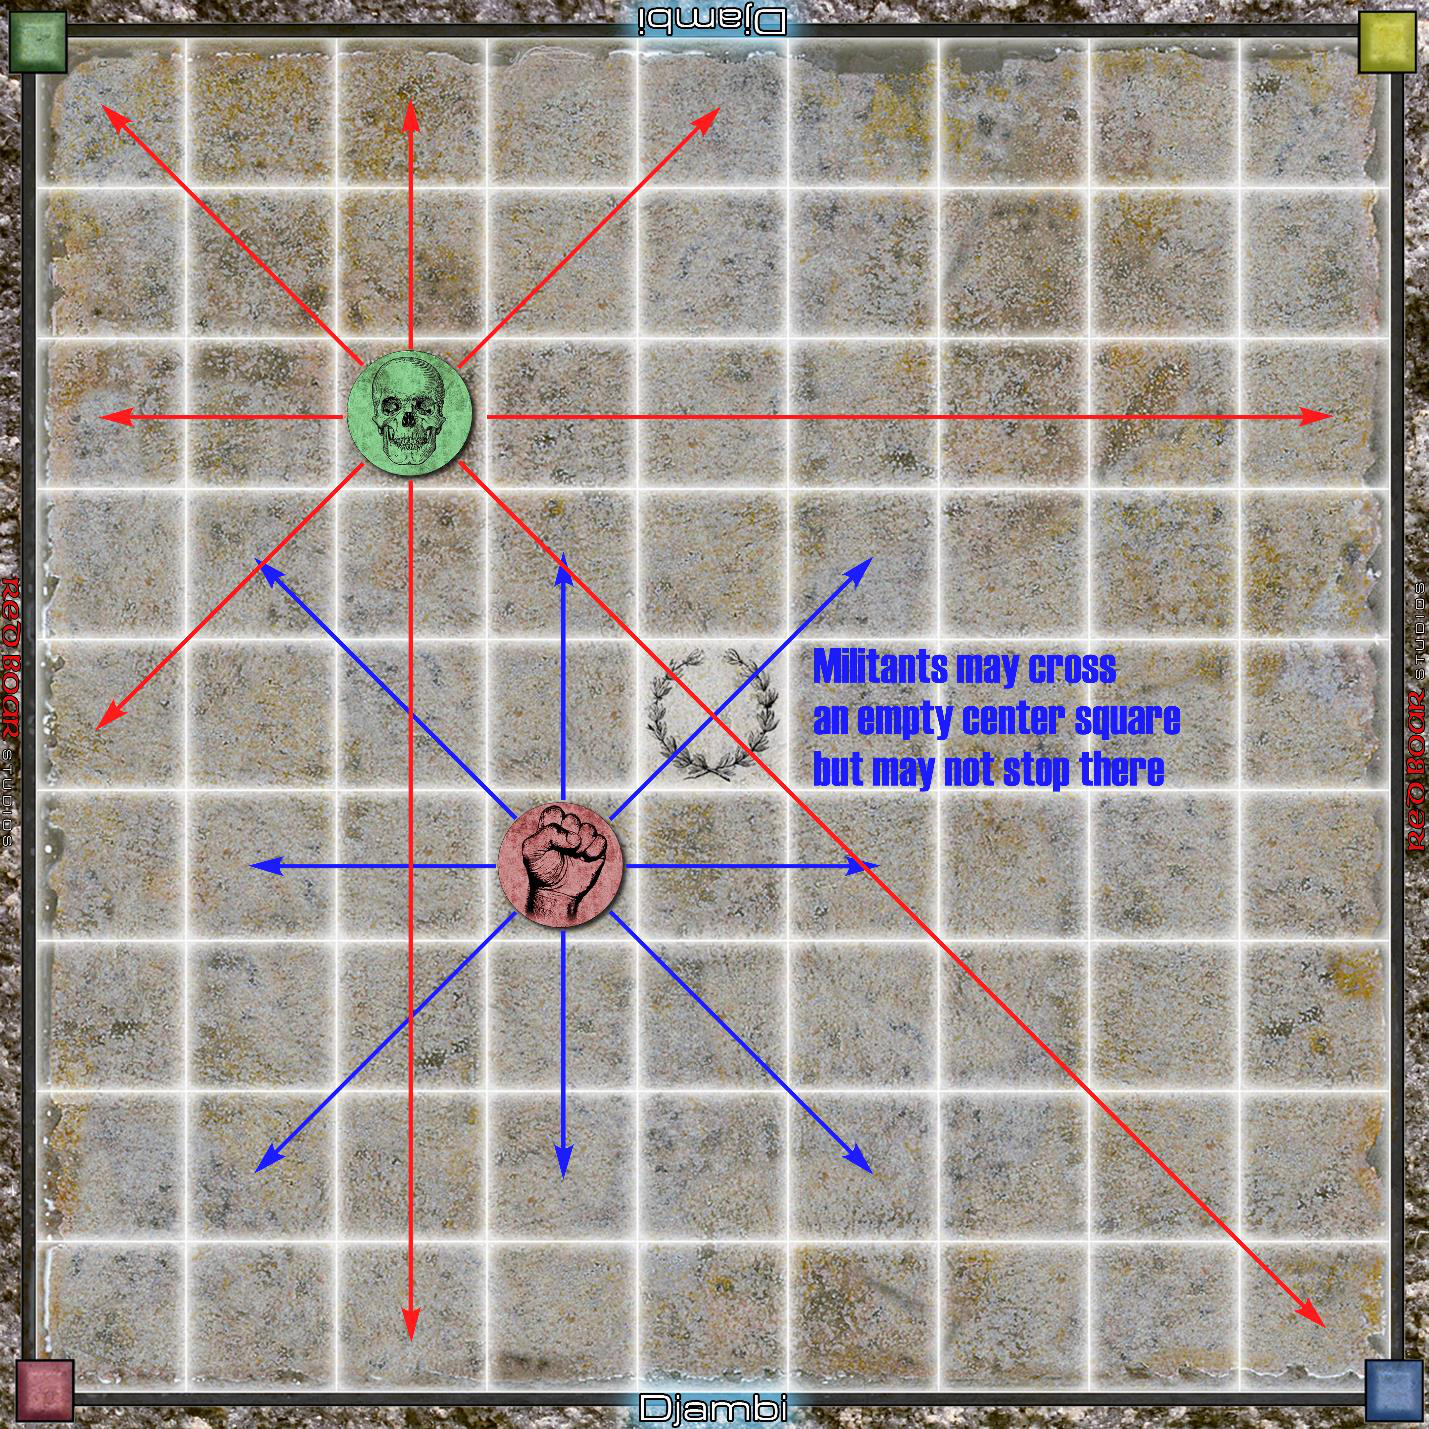
\includegraphics[width=4in,height=4in]{media/image2.png}
\caption{Déplacement d'un militant et d'un necromobile.}
\end{figure}
    

\end{center}

\newpage

\subsection{Effet des pièces}
4 pièces peuvent tuer: le militant, le chef, l'assassin et le reporter. Les pièces éliminées sont replacées sur le plateau face verso.
2 autres pièces ne peuvent tuer mais peuvent déplacer leur victime.
\vspace{20pt} % Ajoute un espace avant la citation, ajustez la valeur selon vos besoins


\subsubsection{Le Militant}
Le militant se place sur l'emplacement de sa victime. Celle-ci est alors disposée retournée sur n'importe quelle case libre (sauf la case centrale) du plateau 
par le joueur ayant fait l'action. Une pièce retournée ne peut pas être traversée.


\vspace{10pt} % Ajoute un espace avant la citation, ajustez la valeur selon vos besoins
\noindent % Empêche l'indentation de la ligne
\begin{minipage}{0.3\textwidth} % Ajustez la largeur selon vos besoins
\includegraphics[width=1.5in,height=1.5in]{media/image10.png}
\end{minipage}%
\hfill % Ajoute un espace entre les deux minipages
\begin{minipage}{0.75\textwidth} % Ajustez la largeur selon vos besoins

\begin{quote}
\textit{These eternal sacrificers advance with counted steps. The Militant has a
course limited to two squares (minimum one square). The Militant can
cross the empty Labyrinth. Their limited march makes them tools that
parties use happily, alive for mischief or dead as martyrs.
These unheralded but courageous and dedicated activists to the Cause can
kill any piece on the field, including a Leader.}
\end{quote}
\end{minipage}
\vspace{20pt} % Ajoute un espace avant la citation, ajustez la valeur selon vos besoins



\subsubsection{Le Chef}
Le chef tue comme un militant. S'il meurt, le joueur est éliminé.

\vspace{10pt} % Ajoute un espace avant la citation, ajustez la valeur selon vos besoins
\noindent % Empêche l'indentation de la ligne
\begin{minipage}{0.3\textwidth} % Ajustez la largeur selon vos besoins
\includegraphics[width=1.5in,height=1.5in]{media/image13.png}
\end{minipage}%
\hfill % Ajoute un espace entre les deux minipages
\begin{minipage}{0.75\textwidth} % Ajustez la largeur selon vos besoins

\begin{quote}


\textit{The Leader is the most important piece on the board for a player's
party. Should he be lost, the game is lost. The first great irony is
that he must risk exposure in order to gain superior power against the
other parties.
The Leader can kill any piece occupying the field, then returns his
victim's corpse to any free square on the board where the
placement benefits the party\textquotesingle s interest.
}
\end{quote}
\end{minipage}
\vspace{20pt} % Ajoute un espace avant la citation, ajustez la valeur selon vos besoins


\newpage


\subsubsection{L'Assassin}
L'assassin se place également sur la case de sa victime, mais ne choisit pas l'emplacement du mort: celui-ci est placé à la case d'origine de l'assassin.

\vspace{20pt} % Ajoute un espace avant la citation, ajustez la valeur selon vos besoins
\noindent % Empêche l'indentation de la ligne
\begin{minipage}{0.3\textwidth} % Ajustez la largeur selon vos besoins
\includegraphics[width=1.5in,height=1.5in]{media/image8.png}
\end{minipage}%
\hfill % Ajoute un espace entre les deux minipages
\begin{minipage}{0.75\textwidth} % Ajustez la largeur selon vos besoins

\begin{quote}
\textit{
As the name suggests, he may kill any enemy piece. But he cannot
disguise his crime by placing the corpse wherever it seems beneficial to
him on the ground. Instead, his victim takes his place from which he
started his move. A powerful instrument, the Assassin leaves traces and
When the Assassin kills, he takes the place of a coin and the one killed
is then placed in the starting square from where the Assassin moved
from.}
\end{quote}
\end{minipage}
\vspace{25pt} % Ajoute un espace avant la citation, ajustez la valeur selon vos besoins

\begin{figure}[ht]
\centering
\includegraphics[width=5in,height=4in]{media/image9.png}
\caption{L'assassin rouge élimine le militant vert.}
\end{figure}
\newpage

\subsubsection{Le Reporter}
Le reporter tue en se plaçant sur une case adjacante (diagonale non comprise) à sa victime. Celle-ci est alors retournée en restant à sa place. 
Le reporter ne peut tuer qu'après un déplacement de sa part.


\vspace{5pt} % Ajoute un espace avant la citation, ajustez la valeur selon vos besoins
\noindent % Empêche l'indentation de la ligne
\begin{minipage}{0.3\textwidth} % Ajustez la largeur selon vos besoins
\includegraphics[width=1.5in,height=1.5in]{media/image11.png}
\end{minipage}%
\hfill % Ajoute un espace entre les deux minipages
\begin{minipage}{0.75\textwidth} % Ajustez la largeur selon vos besoins

\begin{quote}
\textit{A living embodiment of scandal, the Reporter does not kill directly, it
splashes destruction round about. The Reporter can only act after a
trip. When he has finished his course, he can at that point annihilate
an opponent\textquotesingle s piece that is on one of the four squares
that have a common side with the one he occupies. The Reporter does not
take the place of the killed piece, and the victim's corpse is not
moved.}
\end{quote}
\end{minipage}

\begin{figure}[ht]
\centering
\includegraphics[width=4.75972in,height=4.76111in]{media/image12.png}
\caption{Le reporter élimine l'une des pièces adjacantes à sa case d'arrivée.}
\end{figure}
\newpage


\subsubsection{Le Diplomate}
Le diplomate peut déplacer une pièce ennemie en vie sur n'importe quelle case libre (sauf case centrale).

\vspace{5pt} % Ajoute un espace avant la citation, ajustez la valeur selon vos besoins
\noindent % Empêche l'indentation de la ligne
\begin{minipage}{0.3\textwidth} % Ajustez la largeur selon vos besoins
\includegraphics[width=1.5in,height=1.5in]{media/image4.png}
\end{minipage}%
\hfill % Ajoute un espace entre les deux minipages
\begin{minipage}{0.75\textwidth} % Ajustez la largeur selon vos besoins

\begin{quote}
\textit{The Provocateur does not kill: he is a manipulator, a mover of the
living. The Provocateur takes the place of a living piece not belonging
to his own camp. The piece taken is placed without being killed, so
remaining alive and able to subsequently act, on any free square of the
field, where the placement benefits the party\textquotesingle s
interest. The Provocateur cannot, in this game, manipulate his own
parties' pieces.}
\end{quote}
\end{minipage}

\begin{figure}[ht]
\centering
\includegraphics[width=4.75972in,height=4.76111in]{media/image5.png}
\caption{Le diplomate bleu déplace l'assassin jaune à proximité du chef vert}
\end{figure}
\newpage


\subsubsection{Le Necromobile}
Le Necromobile peut déplacer un mort sur n'importe quelle case libre (excepté la case centrale).

\vspace{5pt} % Ajoute un espace avant la citation, ajustez la valeur selon vos besoins
\noindent % Empêche l'indentation de la ligne
\begin{minipage}{0.3\textwidth} % Ajustez la largeur selon vos besoins
\includegraphics[width=1.5in,height=1.5in]{media/image6.png}
\end{minipage}%
\hfill % Ajoute un espace entre les deux minipages
\begin{minipage}{0.75\textwidth} % Ajustez la largeur selon vos besoins

\begin{quote}
\textit{The Necromobile does not kill: he is a salvager, a mover of the dead. He
uses, for the benefit of his party, any corpse lying on the ground,
taking its place. The corpse is then placed, remaining dead without the
possibility of zombie animation or network syndication, on any free
square of the field, where the placement benefits the
party\textquotesingle s interest. A corpse can be either an obstacle or
a guarantee.}
\end{quote}
\end{minipage}

\begin{figure}[ht]
\centering
\includegraphics[width=4.75972in,height=4.76111in]{media/image7.png}
\caption{Le Necromobile rouge déblace un mort pour bloquer l'assassin bleu.}
\end{figure}
\newpage





\subsection{Elimination d'un joueur}
Un joueur est éliminé lorsque son chef meurt. Cela peut arriver de 2 façons différentes:

\subsubsection{Mort directe}
Un chef peut être éliminé directement par un autre joueur (avec un militant, un reporter, un assassin ou un autre chef).


Toutes les pièces restantes du joueur éliminé deviennent alors contrôlées par le joueur auteur de l'élimination et sont considérées comme des pièces alliées.
(pas d'action possible du dimplomate du joueur sur elles et inversement). A son tour, le joueur peut décider de jouer indistinctement une de ses pièces ou une pièces alliée.

\subsubsection{Mort par encerclement}
Un chef peut être éliminé par encerclement si ni lui ou ni aucune de ses troupes adjacentes de proche en proche ne peut se déplacer.
Cela signifie en général que le groupe de pièces est entourée de morts (sauf pour le necromobile qui peut alors encore se déplacer sur un mort).

Le joueur est alors éliminé et le jeton de son chef est retourné. Toutes ses pièces encore en vie sont désactivées: les autres joueurs ne peuvent ni les tuer, ni les déplacer jusqu'à ce qu'elles soient ralliées par un chef au pouvoir (cf section suivante, prise de pouvoir).

\subsubsection{Fin de partie}
La partie se termine lorsqu'il ne reste plus qu'un seul joueur en jeu ou lorsqu'un joueur au pouvoir ne peut plus être éliminé (cf intouchable et forteresse, sections suivantes).
Celui-ci est alors déclaré vainqueur.
Si les joueurs ne peuvent se départager, la partie est déclarée nulle et il n'y a pas de vainqueur.


\newpage

\subsection{Prise de pouvoir}
La case centrale ne peut être occupée par aucune autre pièce que le chef.
Lorqu'un chef se déplace sur la case centrale, on dit qu'il "prend le pouvoir": le joueur en tire de nombreux bénéfices et peut même se voir offrir un nouveau chemin vers la victoire.
Voici les effets:


\subsubsection{Soumission des pièces neutres}
Toutes les pièces qui ont été désactivées (suite à l'encerclement d'un chef) passent définitivement sous le contrôle du chef au pouvoir en tant que pièces alliées.

Si un joueur se fait éliminer par encerclement alors qu'un autre joueur est encore au pouvoir, ses pièces restantes passent automatiquement et définitivement sous le contrôle du joueur au pouvoir.

\subsubsection{Droit de Réponse}
Le joueur au pouvoir joue après chacun de ses adversaires tant qu'il reste au pouvoir. Il joue donc autant de fois qu'il a d'adversaires.

S'il quitte le pouvoir lors de l'un de ses tours, il doit attendre un tour complet avant de rejouer (changement possible dans l'ordre de jeu des joueurs).

S'il se fait démmettre du pouvoir par un reporter, il joue un tour complet après son dernier tour joué (même effet qu'au dessus).

\subsubsection{Intouchable}
Un chef au pouvoir ne peut être éliminé directement par un militant.

Si aucun joueur ne peut éliminer le chef au pouvoir (par exemple s'il n'y a plus d'autre pièce ennemie capable de l'atteindre qu'un autre chef), celui-ci est déclaré vainqueur.

\subsubsection{Forteresse}
Un chef au pouvoir ne peut être éliminé par encerclement. 

S'il est encerclé et qu'aucun autre joueur n'est capable de défaire cet encerclement (par exemple s'il n'y a plus de necromobile ennemi encore en jeu), 
le chef au pouvoir devient alors impossible à destituer et gagne la partie.



\newpage

\subsection{Elimination d'un chef au pouvoir}
Si sa prise de pouvoir n'a pas été anticipé, il peut être très difficile de neutraliser un chef au pouvoir.
Voici les possibilités:

\subsubsection{Elimination par un autre chef}
Le cas est peu fréquent s'il n'est pas anticipé. Le chef tueur prend alors la place au centre, prend le pouvoir et le contrôle de toutes les pièces du joueur éliminé comme de ses pièces alliées.

\subsubsection{Elimination par un reporter}
Un reporter se place à côté du chef au pouvoir et le tue. La pièce du chef retournée reste au pouvoir et bloque les prochains prétendants. Seul un necromobile pourra venir le déloger.

\subsubsection{Elimination par un assassin}
Une fois sur la case centrale, l'assassin ne peut y rester et rejpue immédiatement pour en sortir. S'il tue une autre pièce lors de son second tour, il doit placer le corps du jeton éliminé sur la case
centrale comme dans le cas précédent. Il prend le contrôle de toutes les pièces du joueur éliminé et des ses éventuels alliés.

\subsubsection{Neutralisation par un diplomate}
Un diplomate peut venir déloger le chef au pouvoir. Ne pouvant rester sur la case centrale, il rejoue immédiatement pour sortir de la case centrale.

\subsubsection{Action du necromobile}
S'il y a un mort au pouvoir, à cause d'une action du reporter ou de l'assassin, le necromobile peut venir le déloger et rejoue dans la foulée.

\newpage


\section{Règles Avancées}

Les règles ont été adaptées pour permettre de jouer à 6 joueurs.
Ces règles se jouent sur un plateau hexagonal. Elles demandent encore plus de diplomatie et de stratégie pour gagner.

\vspace{20pt} % Ajoute un espace avant la citation, ajustez la valeur selon vos besoins


\begin{figure}[ht]
\centering
\includegraphics[width=4.75972in,height=4.76111in]{media/dja_6_tablier.png}
\caption{Placement des pièces en début de partie sur le plateau hexagonal.}
\end{figure}


\newpage

\vspace{30pt}

\subsection{Evolution du plateau}

Le plateau est hexagonal et comporte donc 6 coins. Chaque joueur dispose de 9 pièces disposées dans chaque coin du plateau.

\subsubsection{Déplacements}

Le déplacement des pièces est similaire à la version classique: en lignes droites et en diagonales. Le nombre de directions possibles passe de 8 à 12.

Les pièces se déplacent sans limite de portée sauf pour les militants qui ont une portée de 2 cases en ligne droite et 1 case en diagonale.
Une pièce ne peut traverser une case occupée.

\vspace{10pt}

\begin{figure}[ht]
\centering
\includegraphics[width=5in,height=3.1in]{media/dja_6_01.png}
\caption{Déplacements sur le plateau hexagonal à 6 personnes.}
\end{figure}

\subsubsection{Case centrale}

Seul un chef peut occuper la case centrale. De la même manière qu'aux règles classiques, une pièce simple qui vient de déloger un chef doit rejouer immédiatement pour en sortir.

Si un chef est au pouvoir, les 6 cases autour de lui sont réservées à ses troupes ou alliés.
Une pièce exterieure ne peut venir s'y placer que pour y faire une action (tuer ou déplacer) et doit rejouer immédiatement pour en sortir (vers l'exterieur).

Si des pièces ennemies sont sur ces cases avant qu'un chef prenne le pouvoir, elles sont éliminées et placées retournées sur ces mêmes cases.

\newpage

\subsection{Evolution des pièces}

4 pièces voient leur champ d'action renforcé: l'assassin, le reporter, le diplomate et le necromobile. Ces 4 pièces deviennent particulièrement précieuses pour arracher la victoire.

Cette évolution des pièces est permise dans une partie à 6 joueurs car s'il est bien plus facile d'y éliminer une pièce adverse, le faire par le sacrifice d'une pièce alliée n'est pas un choix anodin:
ce ne sont plus 2 autres joueurs qui profitent de ces pertes, mais 4.
Il n'est donc recommandé de sacrifier vos pièces que lorsque le jeu en vaut la chandelle.

\subsubsection{L'Assassin}
L'assassin peut maintenant traverser les pièces alliées.

Il devient une pièce redoutable, qui ne prend pas de risque inutile et vise des cibles importantes.
Il collabore bien avec les militants qui sont légions en début de partie, mais est aussi utile en fin de partie pour débusquer un chef au pouvoir difficile à approcher.

\subsubsection{Le Reporter}
Le reporter élimine maintenant toutes les pièces ennemies qui l'entoure (sur les 6 cases adjacentes) à chaque déplacement de son initiative.
Il est aussi autorisé à aller sur la case centrale pour tuer (une pièce ennemie doit donc être présente sur une des 6 cases autour) mais doit rejouer immédiatement pour en sortir.

Le reporter rêve du scoop qui décimera des gangs entiers et n'hésitera à profiter des services d'un diplomate véreux pour s'y infiltrer.

\subsubsection{Le Diplomate}
Il peut maintenant déplacer les pièces alliées en dehors du chef et du necromobile.

Le diplomate devient encore plus redoutable en début de partie car il permet au joueur d'organiser son jeu.

\subsubsection{Le Necromobile}
Il peut maintenant traverser les morts.

Toujours aussi vulnérable et encombrant en début de partie, il devient insaisissable en fin de jeu, un véritable enfer pour ses adversaires et un atout clé pour la victoire.

\subsubsection{Le Militant}
Le militant peut maintenant éliminer directement un chef au pouvoir, comme toutes autre pièce. 
Il doit rejouer immédiatement pour sortir du pouvoir.


\newpage

\subsection{Coups et stratégies usuelles}

Voici quelques astuces et stratégies usuelles utilisées au Djambi à 6 personnes. 
Elles vous permettront, si vous débutez, de ne pas être totalement vulnérable face à des joueurs plus experimentés.

\subsubsection{Stratégies usuelles au pouvoir}

Un chef au pouvoir est d'autant plus puissant qu'il a d'adversaires.
C'est donc ici qu'il applique fidèlement la maxime de Machiavel: diviser pour mieux régner.
Il a en général pour stratégie d'isoler et affaiblir simultanément chacun de ses adversaires simultanément pour que sa suprématie ne puisse être contestée.

Il cherche généralement à éviter que ses adversaires s'éliminent directement entre eux et privilégiera souvent de les étouffer par encerclement pour récupérer 
le contrôle de leurs pièces.
Le necromobile est ainsi probablement la pièce la plus puissante au service du chef au pouvoir. Elle lui permet aussi de batir une forteresse de morts 
capable de lui assurer la victoire.

Le diplomate est également très utile au joueur au pouvoir pour faire assassiner directement de puissants rivaux.


\subsubsection{Stratégies usuelles face au pouvoir}

Le necromobile est aussi un atout majeur pour les joueurs faisant face au pouvoir pour lutter contre une mort par étouffement et la construction d'une forteresse.

Face à un chef au pouvoir encore peu protégé, le reporter sera efficace car il peut l'éliminer en se plaçant sur une des 6 cases autour de la case centrale et n'a donc pas besoin de se placer dans sa ligne de mire.

Face à un chef au pouvoir très protégé en revanche, il est possible que le reporter ne puisse l'approcher. 
L'assassin est alors sans doute la pièce qui puisse le mieux se frayer un chemin jusqu'au chef au pouvoir pour l'eliminer.

Il est conseillé aux joueurs faisant face au pouvoir de ne pas trop se diviser et d'éliminer le plus rapidement le joueur au pouvoir avant que ce dernier ne devienne trop puissant.

\subsubsection{Stratégies usuelles en début de partie}

Presque toutes vos pièces sont vulnérables en début de partie (excepté le chef et l'assassin) et peuvent se faire éliminer avant même votre premier tour.
Votre reporter peut déjà se faire éliminer par un assassin, votre diplomate peut se faire déplacer par un autre diplomate, et votre necromobile peut se faire éliminer par un assassin ou un reporter.

La seule chose susceptible d'empêcher votre adversaire de procéder à une telle aggression en début de partie est que cela le laisse vulnérable face à un autre joueur, ainsi que de se créer un ennemi juré dès le début de la partie.

A 6 personnes, malgré les nombreuses possibilités d'attaques, les joueurs défensifs et opportunistes auront tendance à sortir leur épingle du jeu face aux joueurs très offensifs.
Il est donc conseillé de commencer à organiser son jeu tôt dans la partie pour laisser le moins de vulnérabilités possibles, et protéger en particulier les pièces que vous jugez les plus utiles.

Le début de partie est aussi le moment de semer la discorde chez les joueurs adverses, un rôle allègrement rempli par votre diplomate.

Enfin, il est conseillé de commencer rapidement à surveiller l'accès au pouvoir. Créez un chemin libre pour votre chef jusqu'au pouvoir pour le prendre le moment venu, et placez en embuscade
des pièces pour en empêcher l'accès aux chefs adverses.

\subsubsection{Coups}
Quelques coups usuels en vrac: 
\vspace{5pt} % Ajoute un espace avant la citation, ajustez la valeur selon vos besoins

\textbf{Traîtrise}: Le pouvoir est occupé. Un assassin élimine une pièce alliée au chef au pouvoir située à côté d'elle et de rejouer immédiatement pour ne pas rester sur l'une des 6 case à côté du centre.
En sortant il élimine une autre pièce dont le mort se place au côté du chef au pouvoir.
C'est un coup traître car il participe à la division des adversaires au pouvoir et à la création de la forteresse.


\textbf{Démolition}: Le pouvoir est occupé. Un necromobile vient retirer un corps qui était à côté du chef au pouvoir, et rejoue immédiatement pour sortir des 6 cases à côté du centre.
Il se cache, et continuera son oeuvre de démolition au fil des tours.

\textbf{Scoop royal}: Le reporter prend la case centrale pour éliminer toutes les pièces autour, puis rejoue immédiatement pour faire un autre scoop à sa sortie.

\textbf{Camouflage}: Il peut être interessant de placer un militant proche d'un chef adverse au pouvoir pour l'empêcher d'y placer un mort et aligner votre assassin derrière. 
Si le chef ne peut bloquer sa ligne de mire avec un corps ni l'éliminer, 
il devra alors quitter le pouvoir de lui-même pour ne pas être sa prochaine victime.

\textbf{Appat}: Un autre moyen de débusquer un chef au pouvoir est de placer dans sa ligne de mire un assassin ou un diplomate qui sera lui même protégé par une autre pièce.
Le chef au pouvoir n'a alors pas d'autre solution que de bloquer le coup avec un corps ou de fuir.

\textbf{Bunker}: Un chef hors du pouvoir peut choisir de s'encercler lui même de morts au côté de son necromobile pour se protéger.
Il n'est alors pas éliminé par encerclement car toutes les pièces encerclées ne sont pas immobilisées (le necromobile peut se déplacer sur un mort).
En revanche s'il n'a plus de pièces à l'exterieur de l'encerclement, il est obligé de déplacer son necromobile car il ne peut passer son tour.

\vspace{10pt} % Ajoute un espace avant la citation, ajustez la valeur selon vos besoins

Il est rappelé que ce jeu est particulièrement injuste, et qu'une défaite n'a pas de signification sur vos compétences de stratège.
\vspace{10pt} % Ajoute un espace avant la citation, ajustez la valeur selon vos besoins

Bon jeu !

\newpage

\subsection{Adaptation du plateau}

Il est possible d'adapter votre Djambi à moins de 6 joueurs. Etant un jeu de diplomatie et de manipulation, il n'est pas interessant d'y jouer à moins de 3 joueurs.

\subsubsection{5 joueurs}

A 5 joueurs, placez les pièces comme pour une partie à 6 joueurs et retournez l'un des chefs: ses troupes sont désactivées.
Elle seront réappropriées par le premier joueur à accéder au pouvoir.

\subsubsection{4 joueurs}

A 4 joueurs, mieux vaut jouer avec le plateau original et les règles classiques.

\subsubsection{3 joueurs}


Le plateau hexagonal à 6 joueurs peut être adapté à 3 joueurs en retirant du jeu les 2 rangées de cases les plus excentrées.
Les règles classiques sont alors utilisées et les pièces ne peuvent se déplacer en diagonale (6 directions seulement).

En effet, les règles avancées sont jugées trop offensives pour une partie à 3 joueurs.

\vspace{5pt} % Ajoute un espace avant la citation, ajustez la valeur selon vos besoins


\begin{figure}[ht]
\centering
\includegraphics[width=3in,height=3in]{media/dja_3_tablier.png}
\caption{Placement des pièces en début de partie sur le plateau hexagonal à 3 joueurs.}
\end{figure}

\vspace{5pt} % Ajoute un espace avant la citation, ajustez la valeur selon vos besoins

Les figures des règles classiques et les paragraphes en italiques associés sont issus de: \textit{Djambi Rules of Play©} 2019 Red Boar Studios.

\end{document}
